\documentclass{article}

\usepackage{graphicx}
\usepackage{geometry}
\setlength{\parindent}{0pt}

\begin{document}

\textbf{Idea}
\\ \\
For our project, we plan to simulate damped, driven pendulums, where both a time-dependent driving force and a damping force dependent on velocity are applied on the pendulum. The user will be able to change physical aspects of the pendulum, as well as swap between a simple pendulum and different physical ones. The motion will be modelled using numerical methods.
\\ \\
\textbf{The Physics} 
\\ \\
With a driving and a damping force, the pendulum's net torque is given by
$$
    \tau_{net} = I \alpha = \tau_{Drive} + \tau_g + \tau_{Drag}.
$$
Since the pendulum is moving through air at relatively high speeds, the drag force is proportional to $v^2$, by a scalar multiple that we will denote $b$. For a simple pendulum with mass $m$ and string length $l$, the net torque becomes 
$$
    \tau_{net} = ml^2 \alpha = lF(t) - mgl\sin(\theta) - blv|v|.
$$
Note that the drag force takes that form because it is always opposite in sign to velocity. Substituting in $l \omega$ for $v$ and isolating $\alpha$, we get
$$
    \alpha = \frac{F(t)}{lm} - \frac{g}{l}\sin(\theta) - \frac{b}{lm}\omega |\omega|.
$$
Thus, the pendulum's motion is modelled by a second-order (nonlinear) differential equation. 
\\ \\
Since the behavior of the pendulum is chaotic, any error will accumulate over time and have a large effect on the motion of the pendulum. We will allow the user to swap between numerical methods of approximation such as Euler's method, where $\omega_k = \omega_{k-1} + \alpha_{k-1} \Delta t$ and $\theta_k = \theta_{k-1} + \omega_{k-1} \Delta t$, and higher-order methods like the Runge-Kutta 4th-order method.
\\
\par
\textbf{UI}
\\ \\
The user will be able to alter sliders to change the mass, string length, starting angle and velocity, drag coefficient, and step size. There will also be dropdown menus for changing the type of pendulum and the approximation method. Furthermore, the user will be able to alter the properties (amplitude, period, phase, etc) of the driving function, as well as choose from several different forms, e.g., $A\cos(bx)$, $A\cos(bx) + C\sin(dx)$, etc.
\\ \\
There will be graphs for angular velocity and acceleration against time, the strength of the driving force against time, kinetic and potential energy against time, as well as a graph for the angular velocity against position in order to visualize attractors.

\newpage
\newgeometry{left=.5in, right=.5in}
\begin{figure}
    \centering
    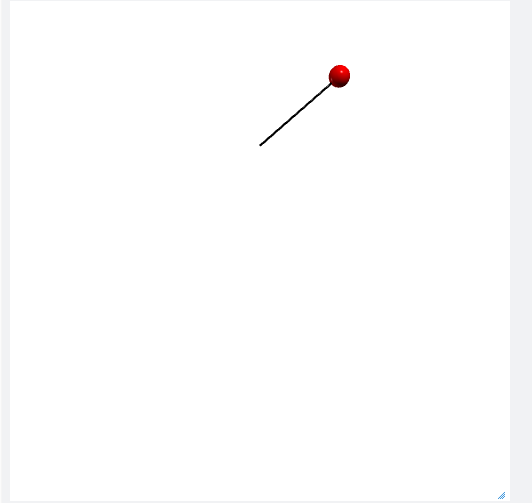
\includegraphics[width=.5\textwidth]{pendulum.png}
    \caption{The Pendulum Display}
\end{figure}

\begin{figure}
    \centering
    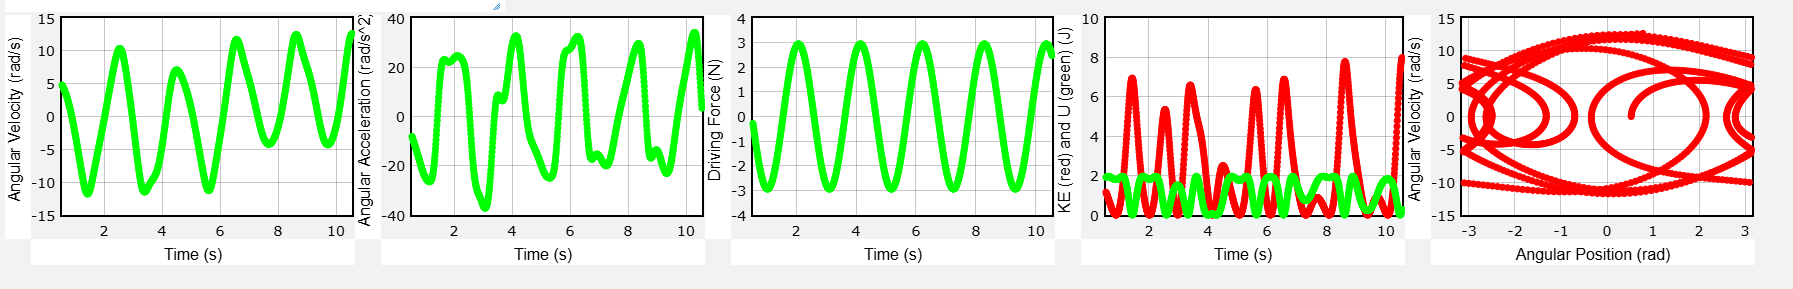
\includegraphics[width=1\textwidth]{graphs.png}
    \caption{The Graphs}
\end{figure}
\end{document}